%----------------------------------------------------------------------------
\section{Model-based Systems Engineering}\label{sec:mbse}
%----------------------------------------------------------------------------

The INCOSE SE Vision 2020\cite{incose-systems-engineering-2020} defines Model-based systems engineering (MBSE) as "the formalized application of modeling to support system requirements, design, analysis, verification and validation activities beginning in the conceptual design phase and continuing throughout development and later life cycle phases. MBSE is part of a long-term trend toward model-centric approaches adopted by other engineering disciplines, including mechanical, electrical and software. In particular, MBSE is expected to replace the document-centric approach that has been practiced by systems engineers in the past and to influence the future practice of systems engineering by being fully integrated into the definition of systems engineering processes."

Applying MBSE is expected to provide significant benefits over the document centric approach by enhancing productivity and quality, reducing risk, and providing improved communications among the system development team.\cite{omgwiki}

In MBSE, one of the most important concepts is the term "model" itself. In the literature it has many different definitions:

\begin{enumerate}
	\item A physical, mathematical, or otherwise logical representation of a system, entity, phenomenon, or process.\cite{DoD_modeling_and_simulation}\label{item:dod}
	\item A representation of one or more concepts that may be realized in the physical world.\cite{sysml_practical_guide}
	\item A simplified representation of a system at some particular point in time or space intended to promote understanding of the real system.\cite{modsim}
	\item An abstraction of a system, aimed at understanding, communicating, explaining, or designing aspects of interest of that system.\cite{object-process-methodology}
	\item A selective representation of some system whose form and content are chosen based on a specific set of concerns. The model is related to the system by an explicit or implicit mapping.\cite{ORMSC/2010-09-06}
\end{enumerate}

As one can see, choosing a definition is very much dependent upon how we wish to use our "model"; in this work I will use the number \ref{item:dod} definition.

\subsection{Systems Modeling Language}

Systems Modeling Language (OMG SysML)\cite{omg_sysml} is a general-purpose modeling language that supports the specification, design, analysis, and verification of systems that may include harware and equipment, software, data, personnel, procedures, and facilities. SysML is a graphical modeling language with a semantic foundation for representing requirements, behaviour, structure, and properties of the system and its components.\cite{sysml_practical_guide}

This work focuses only on the \emph{behavioural} modeling tools SysML provides. In the following section, I present two of the most used concepts.

\subsubsection{State Machine}



\begin{figure}[!ht]
	\centering
	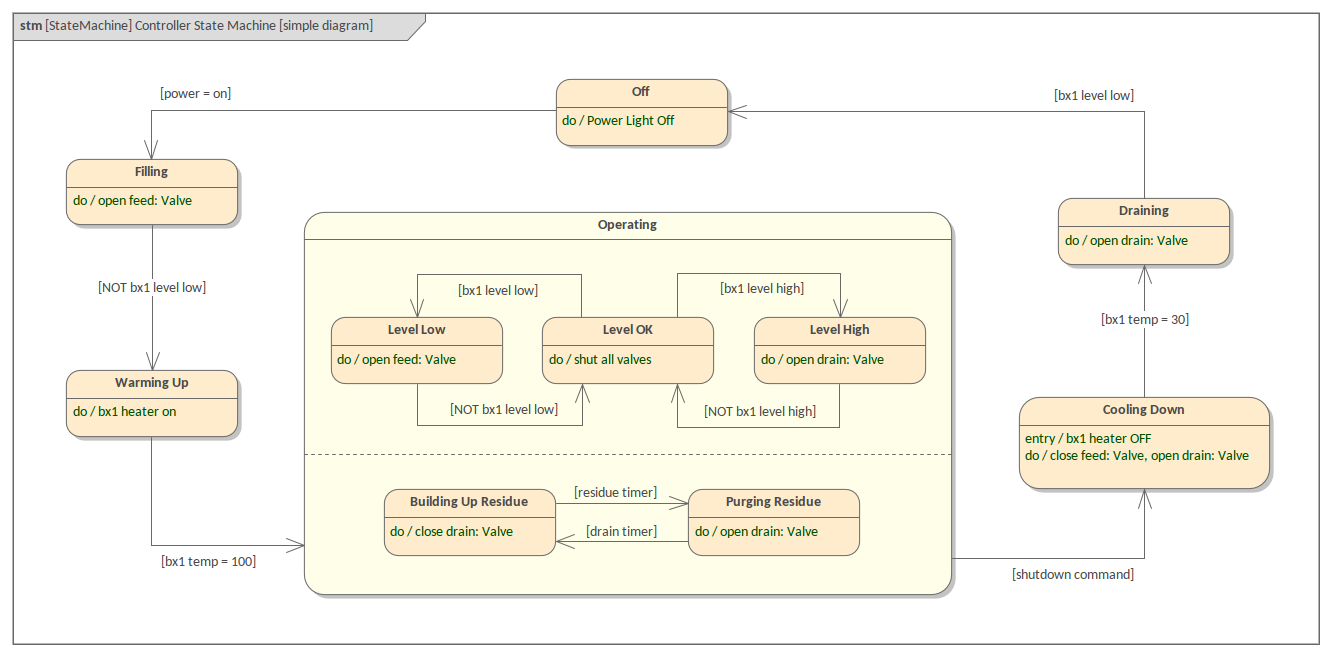
\includegraphics[width=67mm, keepaspectratio]{figures/sysml_state_machine.png}\hspace{1cm}
	\caption{A SysML State Machine.}
	\label{fig:sysml_state_machine}
\end{figure}



\subsubsection{Activity}



\subsubsection{Differences and Combination}

State Machines are a popular [1, 2] language to capture the behaviour
of reactive systems\cite{HAREL1987231} that react to external stimuli depending on
their internal state. Stat Machines provide an expressive formalism to
represent complex \emph{state-based} behaviour by introducing hierarchical
state refinement, memory (variables and history state) and complex
transitions (e.g., fork and join transitions).

As contrast, Activities model the behaviour of distributed systems with many interconnecting components, all running in parallel; said components may have dependencies on each other (one calculates a value the other needs), or have a limited resources (a factory only has one worker).

SysML provides a functionality to combine different behaviours, using the \emph{call behaviour} pattern. By using a call behaviour action inside a State Machine, we are able to combine the behaviour of the two. This is the basis of composite behaviour models, and the motivation of this work. 
